\documentclass[a4paper,12pt,french]{article}

\usepackage[cours]{../../Style}

%\selectcolormodel{cmyk}

%\usepackage{wrapfig}
%\makeatletter
%\setlength{\parskip}{1ex}
%\newcommand{\@minipagerestore}{\setlength{\parskip}{1ex}}

% Début du document
%%%%%%%%%%%%%%%%%%%
\begin{document}

\title{Variables aléatoires}
\maketitle

\begin{programme}
\item Variable aléatoire discrète: Loi de probabilité, espérance
\item Loi de Bernoulli $(0;1)$ de paramètre $p$, espérance
\item Capacités:
\begin{itemize}
\item Interpréter en situation les écritures $\{X=a\}$, $\{X \leq a \}$ et calculer les probabilités correspondantes $\Pro(X=a)$ et $\Pro(X \leq a)$
\item Calculer et interpréter en contexte l'espérance d'une variable aléatoire discrète
\item Reconnaitre une situation aléatoire modélisée par une loi de Bernoulli.
\item Simuler $N$ échantillons de taille $n$ d'une loi de Bernoulli et représenter les fréquences observées des 1 par un histogramme ou un nuage de points
\item Interpréter sur des exemples la distance à $p$ de la fréquence observée des 1 dans un échantillon de taille $n$ d'une loi de Bernoulli de paramètre $p$
\end{itemize}
\item Probabilité associée à une expérience aléatoire à deux épreuves indépendantes
\item Probabilité associée à une répétition d'épreuves aléatoires identiques et indépendante de Bernoulli
\item Capacités
\begin{itemize}
\item Représenter par un arbre de probabilités une expérience aléatoire à deux épreuves indépendantes et déterminer les probabilités des évènements associés aux différents chemins.
\item Représenter par un arbre de probabilités la répétition de $n$ épreuves aléatoires identiques et indépendantes de Bernoulli avec $n \leq 4$ afin de calculer des probabilités
\end{itemize}
\end{programme}

\begin{ex}
On lance pièce équilibrée. Si on tombe sur pile, on gagne 2\euro, sinon on perd 1\euro. On note $X$ les gains après un lancer. Ainsi $X$ peut valoir soit $2$, soit $-1$. La probabilité que $X$ vaille 2, notée $\Pro(X=2)$, vaut $\frac 1 2 = 0,5$.
\end{ex}

\begin{defin}

VAR = fonction $\Omega \rightarrow \R$

\end{defin}

\begin{ex}
\compo[0.58]
{
On reprend l'exemple ci-dessus, mais $X$ représente cette fois les gains après deux lancers successifs. On peut représenter les possibilités grâce à l'arbre ci-contre.

On a alors:
\begin{itemize}
\item  $\Pro(X=1)=\frac 2 4 = 0,5$;
\item $\Pro(X=-2)=\frac 1 4=0,25$.
\end{itemize}
}
{
\begin{center}
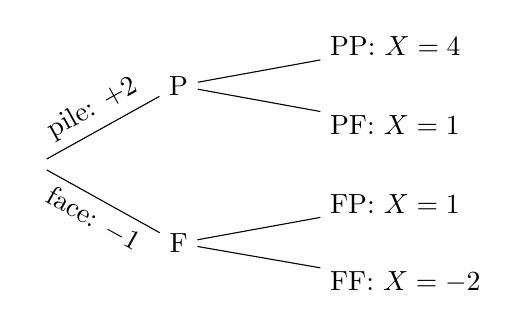
\begin{tikzpicture}[x=1.8cm] % Même effet que xscale=1.8 mais l'option sloped marche

\node (O) at (0,0) {};
\node (P) at (1,1) {P};
\node (F) at (1,-1) {F};
\node[anchor=west] (PP) at (2,1.5) {PP: $X=4$};
\node[anchor=west] (PF) at (2,0.5) {PF: $X=1$};
\node[anchor=west] (FP) at (2,-0.5) {FP: $X=1$};
\node[anchor=west] (FF) at (2,-1.5) {FF: $X=-2$};

\draw (O) -- (P) node[midway,above,sloped] {pile: $+2$} (P) -- (PP) (P) -- (PF) (O) -- (F) node[midway,below,sloped] {face: $-1$} (F) -- (FP) (F) -- (FF);
\end{tikzpicture}
\end{center}
}
\end{ex}

\section{Généralités}
\Def{Soit $\Omega:=\{ \omega_{1},\dots ,\omega_{n} \}$ un ensemble fini qu'on appelle univers. Les $(\omega_{i})$ sont appelés issues possibles.}
\begin{ex}
Pour un lancer de dé à 6 faces on prendra $\Omega=\{ 1,2,3,4,5,6\}$.

\end{ex}
Dans la suite fixons un univers $\Omega$.
\Def{Une \textbf{variable aléatoire} réelle notée $X$ est une fonction de $\Omega \longrightarrow \R$.}

Ainsi, une variable aléatoire c'est affecter à chaque issue possible une valeur.\\
\begin{center}
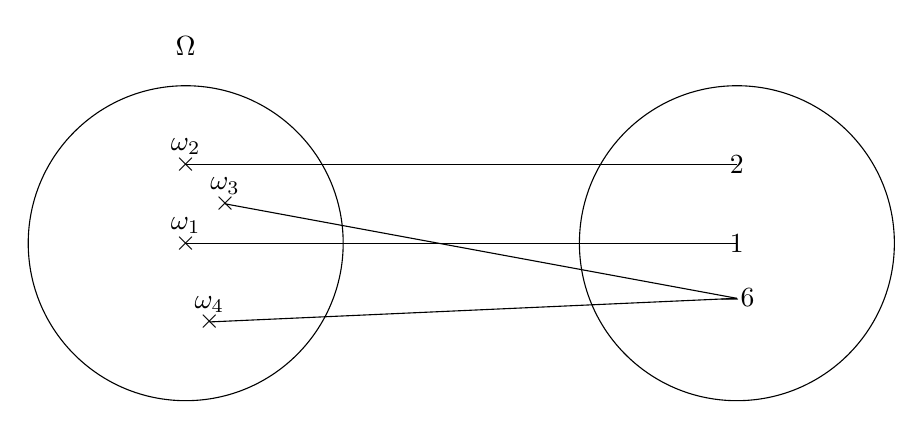
\begin{tikzpicture}
\draw (-2,-2) circle (2cm);
\draw (-2,-2) node{$\times$};
\draw (-2,-2) node[above]{$\omega_{1}$};
\draw (-2,-1) node{$\times$};
\draw (-2,-1) node[above]{$\omega_{2}$};
\draw (-1.5,-1.5) node{$\times$};
\draw (-1.5,-1.5) node[above]{$\omega_{3}$};
\draw (-1.7,-3) node[above]{$\omega_{4}$};
\draw (-1.7,-3) node{$\times$};
\draw (-2,0.5) node{$\Omega$};
\draw (5,-2) circle (2cm); 
\draw (5,-2) node{$1$};
\draw (5,-1) node{$2$};
\draw (5,-2.7) node{$-6$};
\draw (-2,-2)--(5,-2);
\draw (-2,-1)--(5,-1);
\draw (-1.5,-1.5)--(5,-2.7);
\draw (-1.7,-3)--(5,-2.7);
\end{tikzpicture}
\end{center}
\\\\
\underline{Notation:}\\
$\bullet $ L'événement "$X$ prend la valeur $a$" est notée $X=a$.\\ Par exemple, si on reprend la schéma ci-dessus l'évément $X=6$ est réalisé pour les issues $\omega_{3}$ et $\omega_{4}$.\\\\
$\bullet$ L'événement "$X$ inférieur ou égale à $a$" est notée $X\leq a$.\\
Par exemple ici, $X\leq 2$ est obtenue pour les issues $\omega_{2}$ et $\omega_{1}$.
\begin{ex}
On considère un dé à $6$ faces. On associe à chaque numéro des faces une valeur de gain potentielle.
\begin{align*}
    1\longrightarrow -2\euro{}\\
    2,3\longrightarrow -10\euro{}\\
    5\longrightarrow 50\euro{}\\
    4,6\longrightarrow -50\euro{}\\
\end{align*}
Ici, on associe aux issus possibles $\{ 1,2,3,4,5,6 \}$ un élément de l'ensemble $\{ -2,-10,50,-50\}$. On définit ainsi une variable aléatoire $X$.\\
\begin{enumerate}[leftmargin=2cm ]
\item L'événement "$X=-50$" est vérifié pour les issues $4,6$.
\item 
L'événement "$X\leq -10$" est vérifié pour les issues $2,3,1$.
\end{enumerate}
\end{ex}
\begin{de}
Si $X$ est à valeur dans $\{0,1\}$ on parle \textbf{d'épreuve de Bernoulli}.
\end{de}
\begin{ex}
On effectue une épreuve de pile ou face, on peut définir une variable aléatoire $X$ qui a l'événement pile associe 1 et à face 0. Cette variable aléatoire ainsi définie est une épreuve de Bernoulli.
\end{ex}
\section{ Loi de probabilité & Espérance}
\subsection{ Loi de probabilité}
\Def{ Soit $\Omega$ un univers et $X$ une VAR telle que pour tout $i$, $X=a_{i}$ avec $a_{i}\in \R$. \\
Définir la loi de probabilité de $X$, c'est associé à chaque $a_{i}$ la probabilité de l'événement $P(X=a_{i})$.}
Généralement, on relate cela dans un tableau:

\begin{center}
    \begin{tabular}{|p{3cm}|p{3cm}|p{3cm}|p{3cm}|}
    \hline 
       Valeur de $X$ & $a_{1}$ & $\dots$ & $a_{n}$ \\ 
    \hline 
        $ P(X=a_{i})$ & $p_{1}$ & $\dots$ & $p_{n}$\\
    \hline 
    \end{tabular}
\end{center}
\begin{rem}
$P$ étant une probabilité elle doit vérifier $p_{1}+\dots+p_{n}=1$, pour deux événement $A,B$ (c'est-à-dire $A,b\subset \mathscr{P}(\Omega)$) $P(A\cup B)=P(A)+P(B)-P(A\cap B)$ et $P(\emptyset)=0$.
\end{rem}
\begin{ex}
Reprenons l'exemple 2, on a en supposant que le dé est non truqué:\\
\begin{align*}
    & P(X=2)=P(\{ 1 \})=\frac{1}{6}\\
     & P(X=50)=P(\{ 5\} )=\frac{1}{6}\\ 
     
\end{align*}
Comme le dé ne peut tomber sur deux faces en même temps on a donc que $\{4\}\cap \{6\}=\emptyset$ et $\{2\}\cap \{3\}=\emptyset$. Ce qui donne que:
\begin{align*}
    & P(X=-50)= P(\{ 4,6)\})=\frac{2}{6}\\
    & P(X=-10)=P(\{ 2,3\} )=P(\{2\}\cup \{3\})=P(\{2\})+P(\{3\})=\frac{1}{6}+\frac{1}{6}=\frac{2}{6}
\end{align*}
\end{ex}
Que l'on peut répertorier dans le tableau suivant:
\begin{center}
    \begin{tabular}{|p{3cm}|p{3cm}|p{3cm}|p{3cm}|p{3cm}|}
    \hline 
       Valeur de $X$ & $-50$ & $-10$ & $50$ & $2$ \\ 
    \hline 
        $ P(X=a_{i})$ & $\frac{2}{6}$ & $\frac{2}{6}$ &  $\frac{1}{6}$ & $\frac{1}{6}$\\
    \hline 
    \end{tabular}
\end{center}
\subsection{ Espérance, variance et écart type.}
\Def{ En reprenant les notations ci-dessus on définit les notions suivantes: 
\begin{enumerate}[leftmargin=2cm]
    \item \textbf{L'espérance} de $X$ notée $E(X)=a_{1}p_{1}+a_{2}p_{2}+\dots + a_{n}p_{n}$.
    \item \textbf{La variance} de $X$ notée $V(X)=p_{1}(a_{1}-E(X))^{2}+p_{2}(a_{2}-E(X))^{2}+\dots+ p_{n}(a_{n}-E(X))^{2}$
    \item \textbf{L'écart type} $\sigma = \sqrt{ V(X)}$.
\end{enumerate}}
\begin{rem} \hfill \\
$\bullet$ L'espérance traduit le gain moyen lorsqu'on réalise un grand nombre de fois l'expérience aléatoire.\\
$\bullet$ La variance représente la moyenne des carrés des écarts à la moyenne.\\
$\bullet$ L'écart type donne une idée de la dispersion des valeurs de l'échantillon.
\end{rem}
\begin{ex}
Reprenons la loi de probabilité ci-dessus définie par: 
\begin{center}
    \begin{tabular}{|p{3cm}|p{3cm}|p{3cm}|p{3cm}|p{3cm}|}
    \hline 
       Valeur de $X$ & $-50$ & $-10$ & $50$ & $2$ \\ 
    \hline 
        $ P(X=a_{i})$ & $\frac{2}{6}$ & $\frac{2}{6}$ &  $\frac{1}{6}$ & $\frac{1}{6}$\\
    \hline 
    \end{tabular}
\end{center}
Alors on a que:
\begin{align*}
    & E(X)=-50\times \frac{2}{6}-10\times \frac{2}{6}+50\times \frac{1}{6}+2\times \frac{1}{6}=\frac{-100-20+50+2}{6}=\frac{-68}{6}<0
\end{align*}
E(X)<0 donc le jeu n'est pas avantageux puisqu'après un grand nombre de parties on va perdre en moyenne $\frac{-68}{6}$euros soit environs $11$euros.
\end{ex}
\section{La loi de Bernoulli}
\Prop{
Soit $X$ une variable aléatoire suivant une loi de Bernoulli de paramètre $p$ c'est-à-dire que $P(X=1)=p$ alors on a que: $P(X=0)=1-p$ et $E(X)=p$}
\begin{proof}
On sait que $P(X=1)+P(X=0)=p_{1}+p_{0}=p+p_{0}=1$, le résultat est immédiat.\\
De plus, on a que $E(X)=0\times (1-p)+1\times p=p$.
\end{proof}

\end{document}
